%%%%%%%%%%%%%%%%%%%%%%%%%%%%
%\subsubsection{Physics Motivation}
%\label{sec:sp-calib-sys-pns-phys} 

%The supernova signal includes low energy (\SI{10}{\MeV}) electrons, gammas; the final state will also include neutrons visible via capture. Such signals may be sensitive to (local) detector threshold effects, and energy scale, energy resolution; the requirements for these are \SI{0.5}{\MeV}, \SI{1}{\%}, \SI{5}{\%} respectively. 
%\fixme{SG to Jingbo: please make all the edits you have done in SP here as well.}

The \dword{snb} signal includes low-energy  electrons, gammas and neutrons, %the final state will also include neutrons visible via 
which capture on argon. Each signal channel will have specific detector threshold effects, energy scale, and energy resolution. 
As noted in~\physchsnb,
%As noted in the physics volume of the \dword{tdr}, 
the sensitivity to \dword{snb} physics 
%(see Chapter 7 of the \dword{dune} physics \dword{tdr}) 
depends on the uncertainties of relevant detector response parameters, and so a calibration method to constrain those uncertainties is needed.
Local detector conditions may change with time due to a variety of 
%sources,
causes and include electronics noise, misalignments, fluid flow, \dword{lar} purity, electron lifetime, and \efield. While these are intended to be characterized from other systems via inputs to the detector model, ``standard candles'' provide a method to assess if our detector model is incomplete or insufficient. An ideal ``standard candle'' matches one of the relevant signal processes and will provide spatial and/or temporal information. The The \dlong{pns} (\dshort{pns}) system, as described below, will provide a ``standard candle'' neutron capture signal (\SI{6.1}{\MeV} multi-gamma cascade) across the entire \dword{dune} volume that is directly relevant to the supernova physics signal characterization. The \dword{pns} is also capable of providing a spatially fine-grained measurement of electron lifetime. 

%\fixme{SG: this intro needs fixing; our systems are not competing with each other, we need to present them as complimentary systems, so no need to say one is better than the other. I will edit this accordingly so the message is healthy for our maximum benefit.}


%In a TPC the energy reconstruction of a track depends on the amount of charge detected from electrons drifting from the track to the collection plane. For a fixed amount of ionization deposited at a point in the TPC, the amount of charge produced and collected depends on several factors: 
%\begin{enumerate}
%\item The local electric field strength affects the fraction of charge that recombines before drifting. The stronger the field, the less immediate recombination takes place, and thus the ratio of drifting electrons to energy deposited increases.
%\item The electron lifetime depends strongly on the purity of the argon liquid. Given the large size of the DUNE TPC, the restrictions to flow in the active volume, and a likely temperature gradient inside the liquid - it can be expected that there will be parts of the detecter where the electron lifetime will be shorter than others. The prediction of exactly how this manifests is difficult to predict {\it ab initio}.
%\item The distance electroncs have to drift to be collected depends on the location of the vertex inside the volume. The longer the drift, the more likeley it is an electron will be absorbed.
%\item Some parts of the detector can, in principle. be better or worse than others in terms of noise. This can affect the threshold charge collection systematically for different areas or the detector.
%\end{enumerate}

%Given these facts, it is highly desirable to be able to have a "standard candle" energy deposition of known energy that can be detected throughout the volume. Such a standard deposition would reveal variations in the local electron collection efficiency, especially if the source could be triggered such that the $t_0$ of the interaction was known.
%In principle, radioactive sources of known energy distribution could be deployed throughout the detector, but there are several problems with this approach: (1)  the source must be physically placed at the point one wishes to check, requiring multiple deployments in order to sample a significant volume of the detector, (2) the presence of the source itself can alter the electric field and ionization yield, and (3) the introduction of a foreign object into the active volume of the detector carries the risk of introducing impurities and/or radioactive contaminants. In addition, in order to have a triggered source (and hence some idea of $t_0$) one would have to introduce trigger electronics or other instrumentation - further complicating the deployment and increasing the risk.

%A way around this dilemma is to introduce short-lived radioactive atoms into the liquid argon itself, but this has the disadvantage  that there is no trigger and no way to ensure the standard candle decays spread out through the whole volume. In addition, to be useful such isotopes would have to have appreciable half-lives in order to have time to spread around the detector, and thus the whole process might take many hours. Finally, such isotopes would likely need to be made locally, which can be expensive and difficult.

%One way around these issues is to take advantage of a remarkable property of argon - the near transparency to neutrons with an energy near 57 keV due to an anti-resonance in the cross-section caused by the destructive interference between two high level states of the $^{40}$Ar nucleus. 
%As shown in Figure~\ref{fig:Arxsec}, 
%The cross-section at the anti-resonance "dip" is about 10 keV wide, and at the bottom the cross section of $1.6\times 10^{-4}\; b$ implies an elastic scattering length of over $2,000\;m$. Thus to neutrons of this energy the DUNE TPC is essentially transparent, and thus if injected from the top of the detector would reach energy part of the active volume. Of course, natural argon has three major isotopes: $^{36}$Ar (0.3336\%), $^{38}$Ar (0.0834\%), and $^{40}$Ar (99.6035\%) each with a slightly different anti-resonance. \\
%\begin{figure}[h]
%\begin{center}
%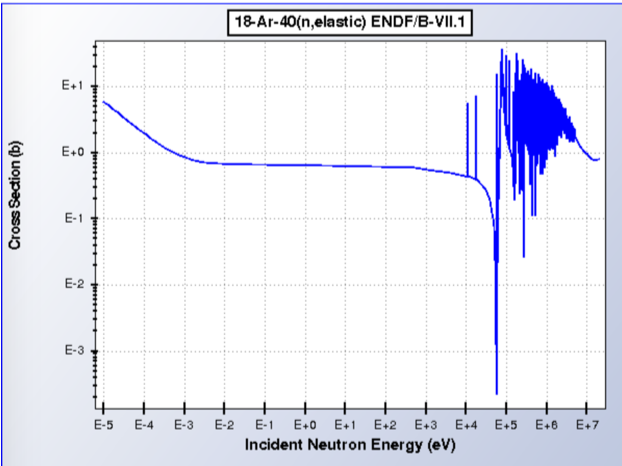
\includegraphics[width=0.4\linewidth]{Figures/Ar40xsec.png}
%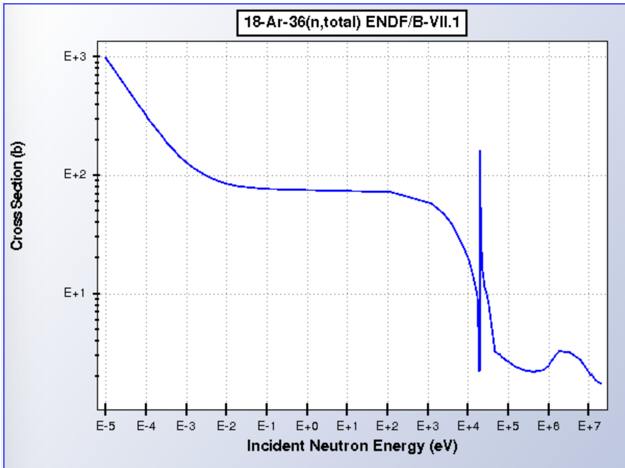
\includegraphics[width=0.4\linewidth]{Figures/Ar36xsec.png}
%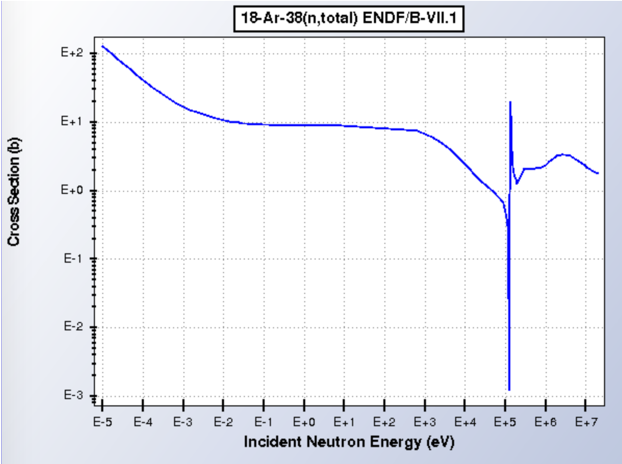
\includegraphics[width=0.4\linewidth]{Figures/Ar38xsec.png}
%\caption{Elastic scattering cross sections on 40-Ar (top left), 36-Ar (top right), and 38-Ar (bottom). From ENDF/B-VII.1~\cite{ref:ENDF}. The large anti-resonance at $57\; keV$ in 40-Ar can be clearly seen.
%{\bf NOTE: PUT IN PLOTS FOR ELASTIC}
%}
%\label{fig:Arxsec}
%\end{center}
%\end{figure}


%\begin{figure}[h]
%\begin{center}
%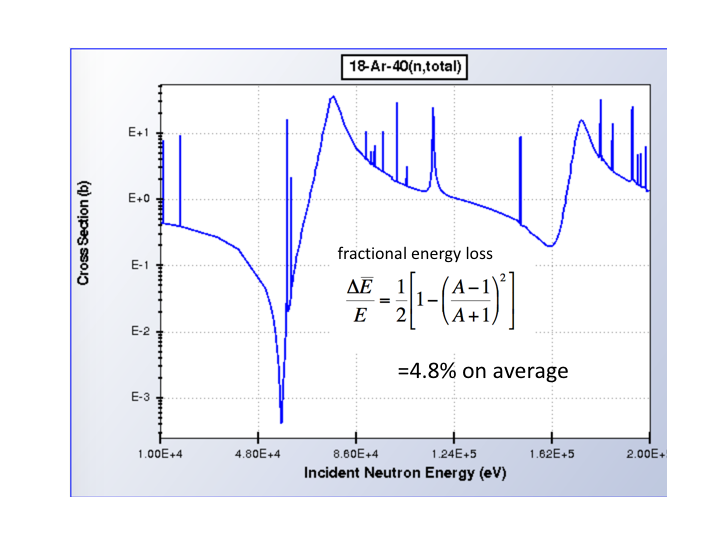
\includegraphics[width=0.75\linewidth]{Figures/Ar40Xsec2.png}
%\caption{Total scattering cross sections on 40-Ar in the range $10-200\; keV$~\cite{ref:ENDF}}
%\label{fig:Arxsec2}
%\end{center}
%\end{figure}

Liquid argon is nearly transparent to neutrons with an energy near or at \SI{57}{\keV} due to an anti-resonance in the cross-section caused by the destructive interference between two high level states of the \argon40 nucleus (see Figure~\ref{fig:PNS_xsections_v2}). The cross-section at the anti-resonance ``dip'' is approximately \SI{10}{\keV} wide, and at the bottom the cross section of \SI{1.6e-4}{\barn} indicates an elastic scattering length of over \SI{2000}{\m}. %Of course, natural 
Natural argon has three major isotopes: \isotope{Ar}{36} (\SI{0.3336}{\%}), \isotope{Ar}{38} (\SI{0.0834}{\%}), and \isotope{Ar}{40} (\SI{99.6035}{\%}) each with a slightly different anti-resonance. The average elastic scattering length of the \SI{57}{\keV} neutrons in natural liquid argon is approximately \SI{30}{\m}.%, dominated by \isotope{Ar}{36}.

\begin{dunefigure}[x-sections enabling the \dword{pns} concept]{fig:PNS_xsections_v2}
{Illustration of interference anti-resonance dips in the cross-section of \isotope{Fe}{56}, \isotope{Si}{28}, \isotope{S}{32}, and \isotope{Ar}{40}. Elastic scattering cross-section data is obtained from ENDF VIII.0~\cite{BROWN20181}.}
%~\cite{Brown:2018jhj}.}
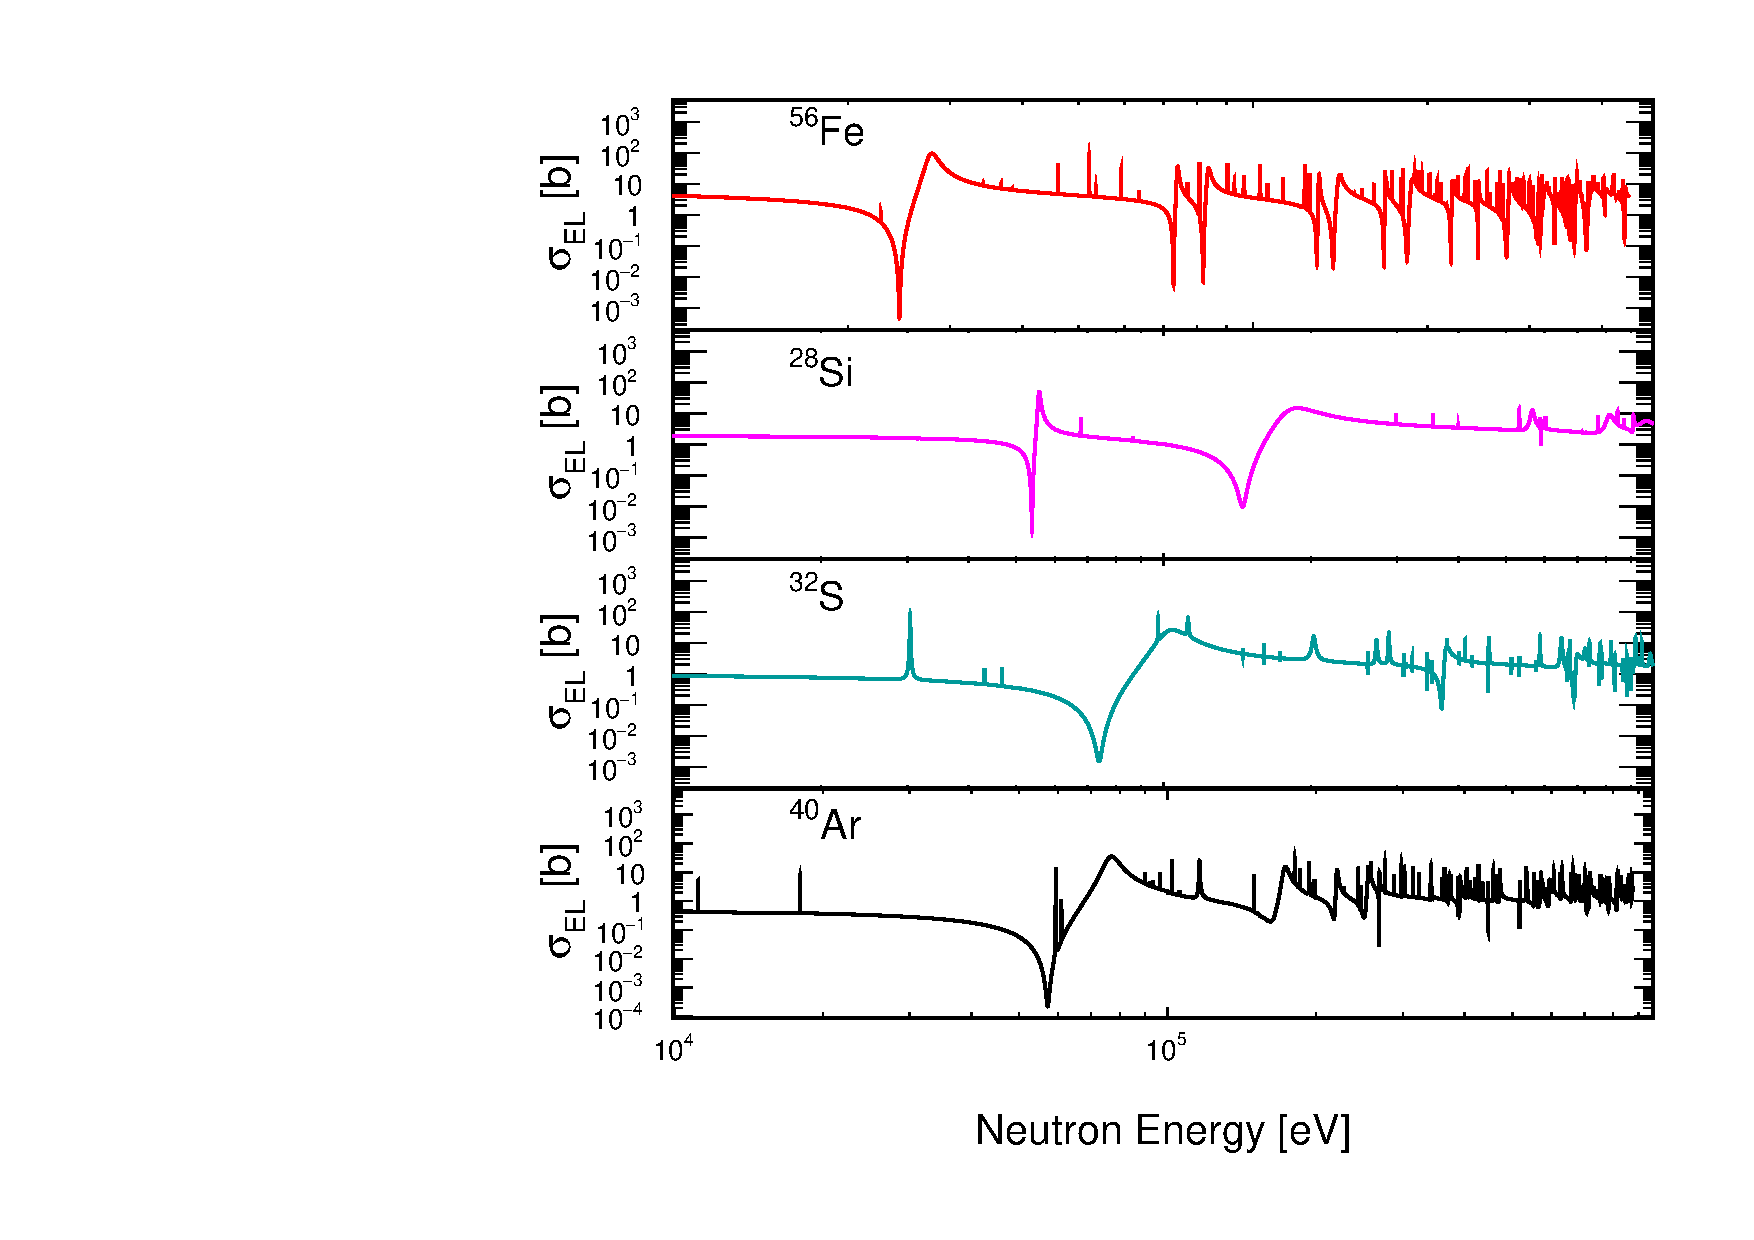
\includegraphics[width=10cm]{graphics/PNS_xsection.pdf}
\end{dunefigure}

The neutrons at the anti-resonance energy could be injected into \dword{lar} in the \dword{tpc}, provided no materials (e.g., hydrocarbons) block the path. Those neutrons that do scatter lose energy, leave the anti-resonance, quickly slow down and are captured. Each capture releases exactly the binding energy difference between \isotope{Ar}{40} and \isotope{Ar}{41}, approximately \SI{6.1}{\MeV}, in the form of $\gamma$ rays. As will be described below, by using a $DD$ generator (where $DD$ stands for ``deuterium-deuterium''), a triggered pulse of neutrons can be generated outside the \dword{tpc}, then injected via a dedicated opening in the insulation into the liquid argon, where it spreads through the \SI{60}{\m} volume of the detector to produce \SI{6.1}{\MeV} energy depositions. %\fixme{Should DD be included among the dwords?}
%Using this method, the calibration procedure would be quick (likely a few hours depending on the neutron yield of the DD generator), and there is no need to manufacture short-lived isotopes at an external facility.

One important property of the neutron capture reaction \isotope{Ar}{40}(n,$\gamma$)\isotope{Ar}{41} is that the deexcitation of \isotope{Ar}{41} nucleus produces a cascade of prompt $\gamma$s. Because of the detector threshold effect, the multiplicity and the
total energy of the $\gamma$s within the cascades could be effectively decreased to below the expected values of the neutron capture process. As a consequence, the neutron capture identification and the assessment of neutron tagging efficiency in liquid argon strongly depends on a precise model of the full $\gamma$ energy spectrum from thermal neutron capture reaction. The neutron capture cross-section and the $\gamma$ spectrum have been measured and characterized by the Argon Capture Experiment at DANCE (ACED). %\fixme{This abbreviation must be defined the first time it is used and included in the general glossary. In fact, this whole sentence has quite a few abbreviations that should be either in the glossary or not used at all.} 
Recently, the ACED collaboration performed a neutron capture experiment using the Detector for Advanced  Neutron  Capture  Experiments (DANCE) facility  at the  Los  Alamos  Neutron  Science  Center (LANSCE). The result of the neutron capture cross-section was published~\cite{Fischer:2019qfr} and will be used to prepare a database for the neutron capture studies. The data analysis of the energy spectrum of correlated $\gamma$ cascades from neutron captures is underway and will be published soon. The $\gamma$ energy spectrum and the branching ratios in the Evaluated Nuclear Data File (ENDF) library will be updated with the ACED result. 

Figure~\ref{fig:PNS_gamma_ACED_v2} shows an example of the energy spectra of individual $\gamma$ clusters measured by ACED~\cite{Fischer:2019qfr}. The most common $\gamma$ cascade emitted from \isotope{Ar}{41} decay has \SI{167}{keV}, \SI{1.2}{MeV} and \SI{4.7}{MeV} $\gamma$s. The peak energy of these $\gamma$s can be clearly seen in the background subtracted data in Ref.~\cite{Fischer:2019qfr}. In liquid argon detectors, the $\gamma$s are detected through calorimetric measurement. Assuming the $\gamma$ cascade from a neutron capture is fully contained in the active volume, it is possible to detect the individual $\gamma$s from the neutron capture. The correlation of the measured $\gamma$ is a strong indication of neutron capture events. Low energy $\gamma$ reconstruction algorithms are being investigated to identify the neutron capture events that could be used for detector response calibration. 

%aced replaced with Fischer:2019qfr
\begin{dunefigure}[Neutron capture gamma spectrum measured by ACED]{fig:PNS_gamma_ACED_v2}
{Energy spectra of individual $\gamma$ clusters measured by ACED. Only events detected in the \SIrange{0.02}{0.04}{eV} neutron energy window are selected.}
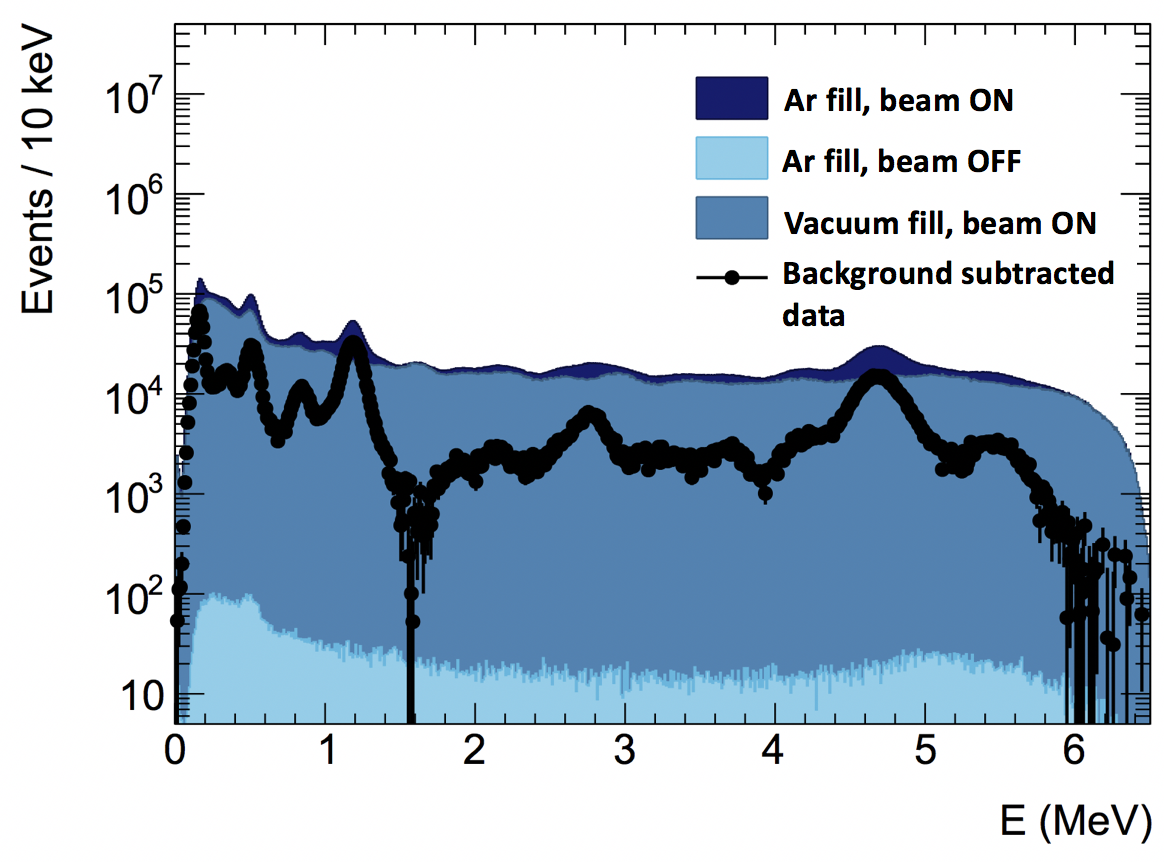
\includegraphics[width=10cm]{graphics/PNS_gamma_ACED_v2.png}
%graphics/PNS_gamma_spectrum_ACED.png}
\end{dunefigure}

%{\it Mention Test at LANSCE and its role?}

%%%%%%%%%%%%%%%%%%%%%%%%%%%%
\subsubsection{Design}
\label{sec:dp-calib-sys-pns-des}

The basic design concept of sources like the \dlong{pns} are based on successful boron neutron capture therapy~\cite{bib:Koivunoro2004}. The design of the \dword{pns} system used for energy calibration is shown in Figure~\ref{fig:PNS_Moderator}. The system will consist of four main components: a $DD$ generator, an energy moderator reducing the energy of the $DD$ neutrons down to the desired level, shielding materials, and a neutron monitor to confirm neutron flux and safe operation. 

\begin{dunefigure}[Conceptual design of the \dlong{pns}]{fig:PNS_Moderator}
{Conceptual design of the \dlong{pns}. The whole device is placed outside the \dword{tpc} volume on top of the cryostat.}
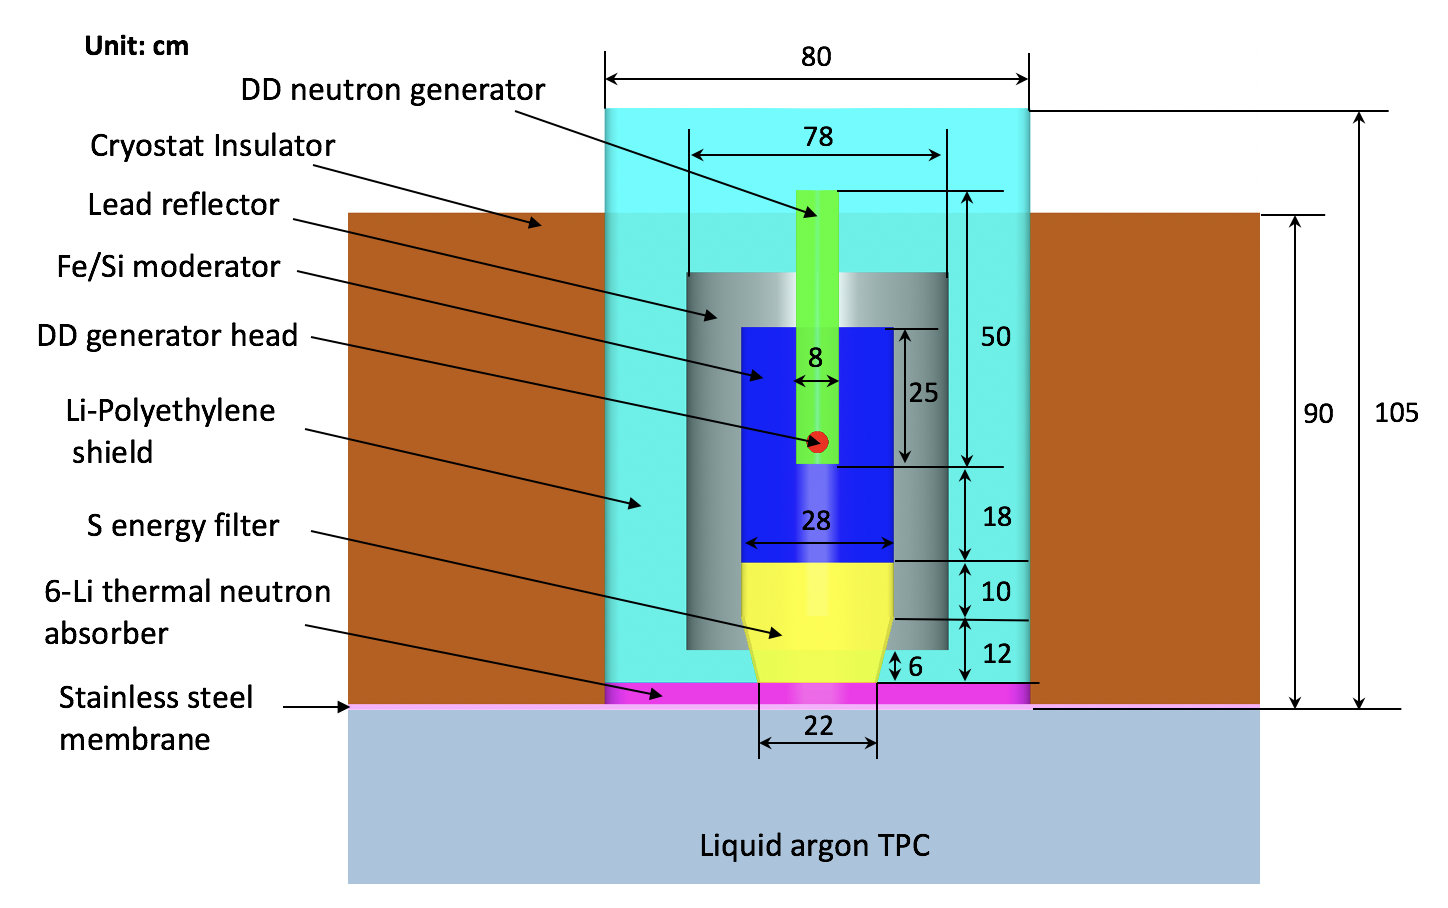
\includegraphics[width=12cm]{PNS_Moderator.png}
\end{dunefigure}

{\bf DD generator source:} %\fixme{This does not appear to be consistent with other similar constructions in the document. I don't know that it matters, but I thought I'd better point it out.} 
$DD$ generators are commercial devices that can be readily obtained from several vendors at a cost of approximately \$\num{125000} each, which includes all control electronics. The pulse width is adjustable and can be delivered from approximately \SIrange{10}{1000}{\micro\s} (which affects the total output). 

{\bf Moderator:}  A feasible moderator has been designed using a layered Moderator~(Fe or Si)-Filter~(S)-Absorber~(Li) %layered 
configuration. The \SI{2.5}{\MeV} neutrons from the $DD$ generator are slowed down to less than \SI{1}{\MeV} by the energy moderator. Natural iron and silicon are found to be efficient moderators for this purpose. Then an energy filter made of sulfur powder further selects the neutrons with the desired anti-resonance energy.
The neutron anti-resonance energy in \isotope{S}{32} is \SI{73}{\keV}, right above the \SI{57}{\keV} anti-resonance energy in \argon40. The neutrons at this energy lose about \SI{3.0}{\keV} per elastic scattering length. After a few elastic scattering interactions, most of the \SI{73}{\keV} neutrons selected by the sulfur filter will fall into the \SI{57}{\keV} anti-resonance energy region in \dword{lar}. These materials require no cooling or special handling. Finally, a thermal absorbing volume of Lithium is placed at the entry to the argon pool to capture any neutrons that may have fallen below the \SI{57}{\keV} threshold. The reflecting volume is added around the $DD$ generator and the neutron moderator to increase downward neutron flux. %Figure~\ref{fig:PNS_Energy_Moderator} shows the energy spectrum of the neutrons moderated and injected into the \dword{tpc}.

%\begin{dunefigure}[Energy of moderated neutrons produced by the %\dshort{pns}]{fig:PNS_Energy_Moderator}
%{Energy of moderated neutrons produced by the \dlong{pns}. %Simulation is based on Design A shown in Figure~\ref{fig:PNS_Two_Designs}. 
%The total number of initial $DD$ generator neutrons is \num{1e6}.}
%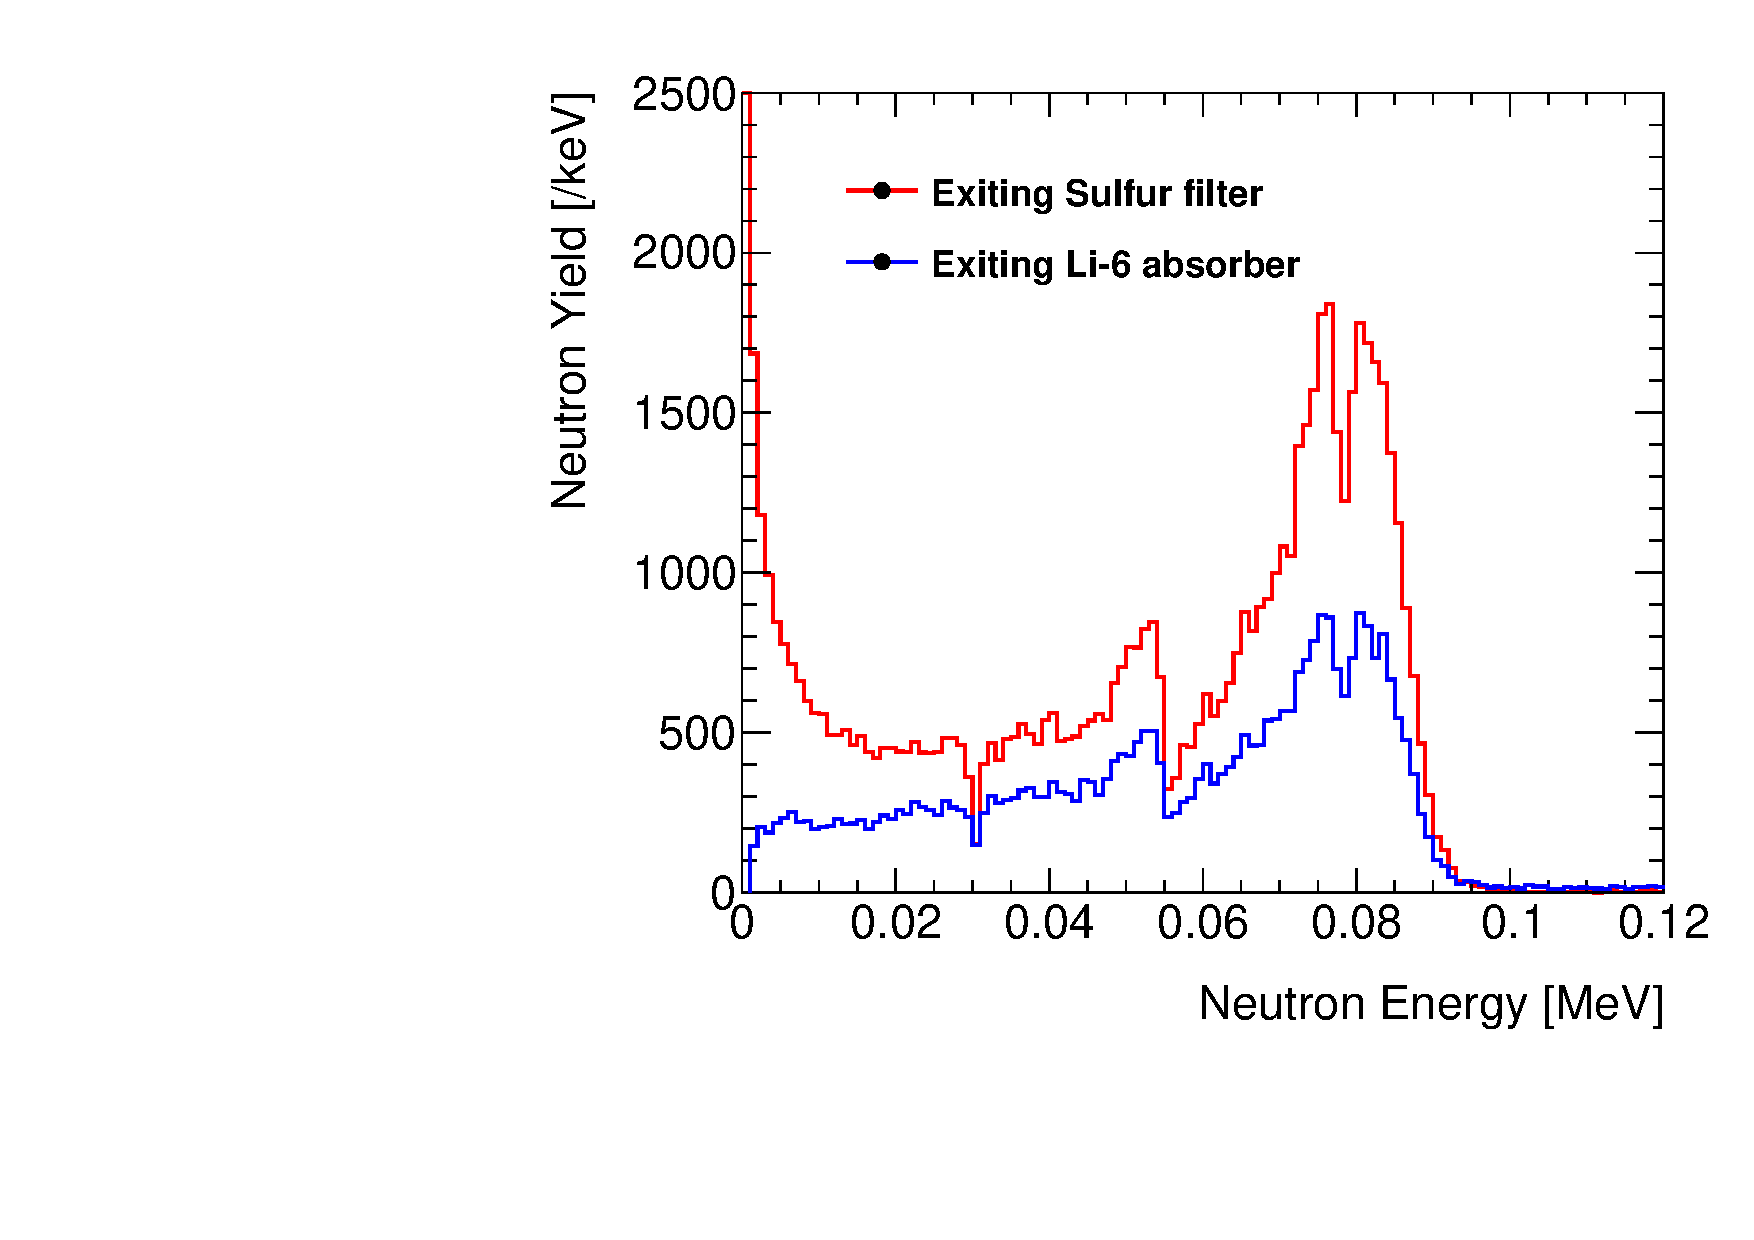
\includegraphics[width=9cm]{PNS_Energy_Moderator.pdf}
%\end{dunefigure}

{\bf Shielding:} The source will be encased in shielding. The goal of the shield is to block both scattered neutrons and gammas produced in the source. Lithium-Polyethylene (\SI{7.5}{\%}) is the material chosen for the neutron shield because it is rich in hydrogen and lithium atoms, which yield a high neutron absorption cross section. Lithium-Polyethylene is also light weight, commercially available, and relatively inexpensive. The energy spectrum entering the shield has several multiple peaks between \SI{0.5}{\MeV} and \SI{1.5}{\MeV}, and one major spike at \SI{2.2}{\MeV}. The shield can effectively block the lower energy peaks but can only degrade the intensity of the \SI{2.2}{\MeV} because \SI{2.2}{\MeV} gammas are a characteristic signature for neutron captures on hydrogen. A safe thickness of the lithium-polyethylene shield must be found, one that can degrade the dose of \SI{2.2}{\MeV} gammas to safe levels. The dose of radiation from \SI{2.2}{\MeV} gammas was calculated assuming a person standing \SI{1}{\m} away. Simulation indicates that a shield with \SI{12}{\cm} thick Lithium-Polyethylene satisfies basic safety requirements\footnote{These calculations will be redone assuming a \SI{30}{\cm} personnel safety distance and shielding thickness reestimated to meet \dword{dune} safety requirements.}. 

{\bf Neutron Monitor:} The system needs a monitoring system to confirm the source is operating as expected.  A neutron monitoring detector consisting of an Eljen EJ-420 coupled to an ADIT L51B16S \num{2}-inch \dword{pmt} will be placed just outside the moderating material surrounding the $DD$ generator and will be read out with a CAEN waveform digitizer with neutron/$\gamma$ pulse-shape discriminating firmware. The monitoring detector will provide relative flux information to the calibration users and will ensure that the intensity of the source is constant, thereby allowing a comparison of data taking at different times.  A small collimator will be placed in front of the neutron detector, inside the shielding material of the $DD$ source. The collimator dimensions and material specifications (likely a combination of iron, lead, and polyethylene) will be optimized from Monte Carlo simulations.

\begin{dunefigure}[Two designs for the \dlong{pns}]{fig:PNS_Two_Designs}
{Two designs being developed for the \dlong{pns}. Design A: Large format neutron source deployed in dedicated neutron injection ports or above/inside the human access ports; Design B: Small format neutron source deployed inside a standard feedthrough port with \SI{25}{\cm} outer diameter.}
%\todo{SG to Jingbo: I have updated the caption for Figure 1.15, please check}
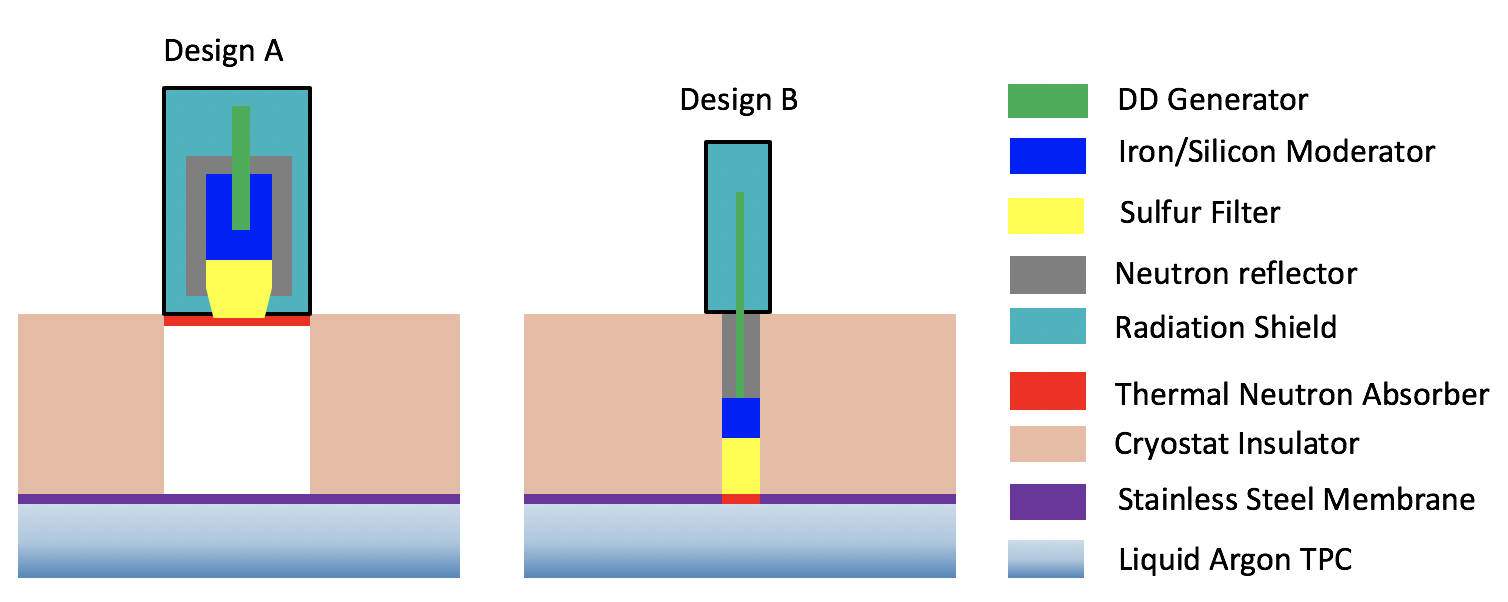
\includegraphics[width=16cm]{PNS_Two_Designs.png}
\end{dunefigure}

Based on the general concept described above, two different designs were studied with GEANT4 simulation. Figure~\ref{fig:PNS_Two_Designs} shows a conceptual layout of the neutron injection system. %\todo{For v2, confirm updated figure; minor error in current one.}

\begin{itemize}
\item {\it Design A: Large format Moderator:} \\
The neutron source is approximately \SI{0.8}{\m} wide and \SI{1}{\m} high. It would sit above the cryostat insulator. Beneath the neutron source, a cylinder insulator volume more than \SI{50}{\cm} in diameter must be removed to allow the neutrons to enter the cryostat. Such an interface is provided by the human access ports near the end-walls of the detector; %Figure~\ref{fig:manhole2} shows a picture of this for \dword{pdsp}. The top flange is sealed, and the neutron source sits on top 
%(Design A), 
%providing heat insulation. 
The neutron source weighs approximately \SI{1.6}{\tonne} and will be supported by the I-beams. This design allows a permanent deployment of the neutron source. GEANT4 simulation has shown that \SI{0.13}{\%} of the neutrons generated by the $DD$ generator should be captured inside the \dword{tpc}. It is also possible to place the neutron source inside the human access ports, which would allow a \num{6}-fold increase of the neutron flux, but this would require modifying the interface flange. This is currently being investigated.
% JW: I think It doesn't harm to mention that the neutron source could be placed inside the manhole. My recent simulation is based on this configuration.

%\item \fixme{KM: I do not think this is possible for quite a few reasons-- heat loss and also cost of adjusting this. Remnoving this for now.} Design B: Large format Moderator; no insulation between Moderator and cryostat membrane The design of the the neutron source itself would be same as Design A. The only difference is that the neutron source will be placed inside a hole on the cryostat insulator. The cryostat will be kept closed, but there is no vacuum insulation between the neutron moderator and the stainless steel membrane. As the neutron source is closer to the liquid argon cryostat, the neutron flux is expected to be a factor of 10 higher than that of Design A. However, the neutron source must be removed and the insulator has to be recovered after the calibration run. 
\item {\it Design B: Small format Moderator:}\\
%no insulation between Moderator liquid argon. 
%An alternative method for delivering the neutrons is to use the existing calibration feedthroughs. In the current cryostat design, \num{20} calibration feedthroughs with a \SI{20}{\cm} inner diameter will be available on top of the cryostat. 
%\todo{SG: Jingbo, check the modification for this. Although we will aim for our ideal ports, it is good to have small format moderator so we have the flexibility to deploy where we think coverage is needed}
The neutron source can be designed with an ultra-thin $DD$ generator that fits a standard-sized feedthrough (\SI{25}{\cm} outer diameter), which permits deploying the neutron source using existing feedthroughs (e.g., instrumentation or other calibration ports). However, the feedthrough has no space for the shielding materials to fit inside, so additional shielding must be placed around the feedthrough. The weight of this compact neutron source will be approximately \SI{140}{\kg}, so mounting would be simpler than in Design A. The effective neutron flux should be similar to Design A. 
\end{itemize}

%\begin{dunefigure}[Flange for human access port on \dword{pdsp}]{fig:manhole2}
%{Flange for human access port on \dword{pdsp} and support structure (red frame).}
%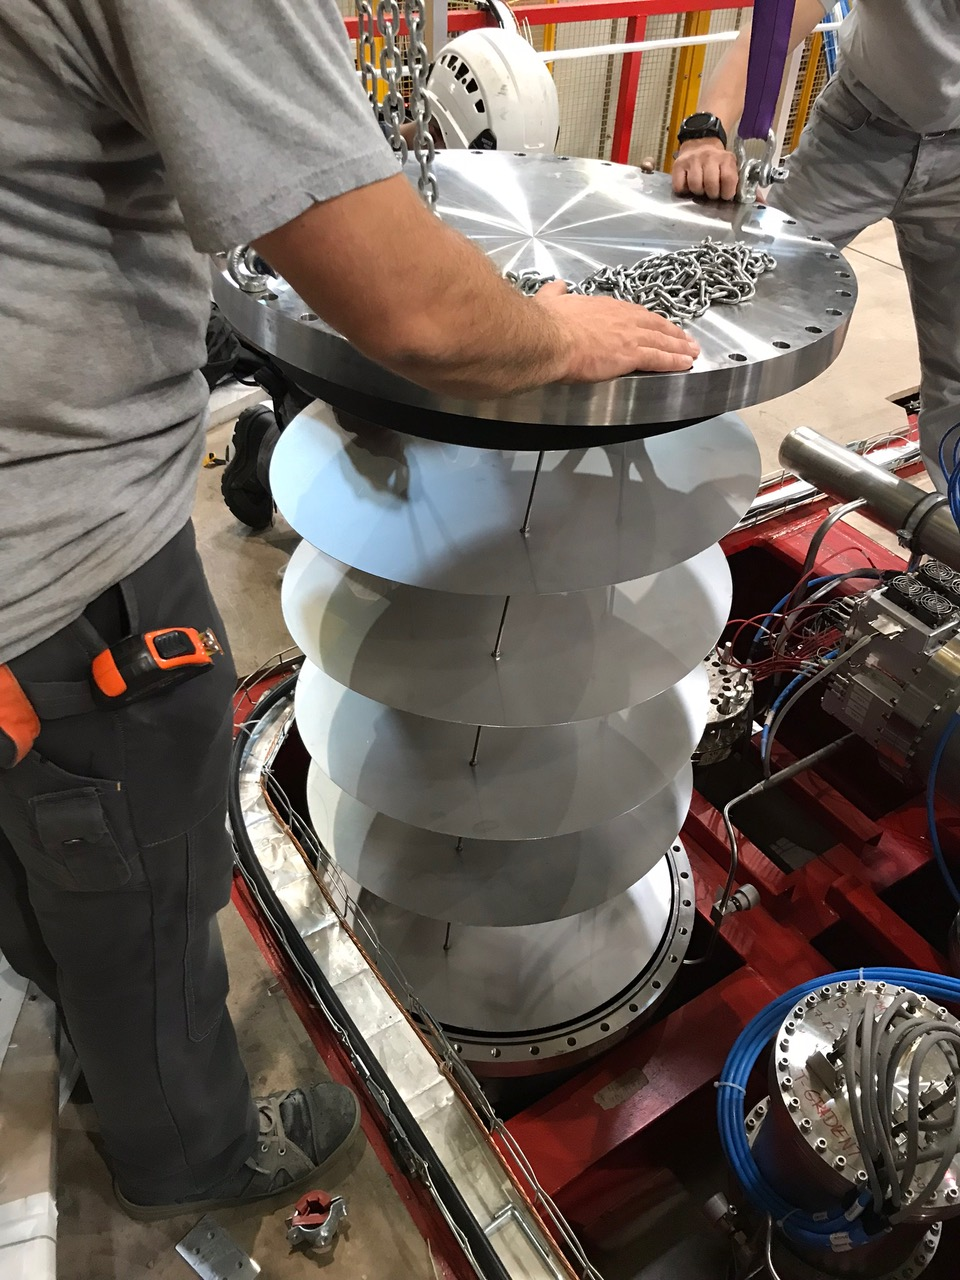
\includegraphics[width=6cm]{manhole2.jpg}
%\end{dunefigure}

\begin{dunefigure}[Pulsed neutron system neutron capture positions inside a \dword{dune}-sized TPC]{fig:PNS_NcapPosition}
{Neutron capture positions inside a \dword{dune}-sized \dword{tpc}. L=\SI{60}{\m} (along $z$ axis, horizontally parallel to the beam direction), W=\SI{14.5}{\m} (along $x$ axis, horizontally perpendicular to the beam direction), H=\SI{10}{\m} (along $y$ axis, vertically perpendicular to the beam direction). The neutron moderator is based on Design A, but the entire source is placed inside the injection port central to the cryostat. \num{1e6} $DD$ generator neutrons with \SI{2.5}{\MeV} energy were simulated in the moderator and propagated inside the \dword{tpc}. Left: Top view of neutron capture positions. Right: Side view of neutron capture positions.}
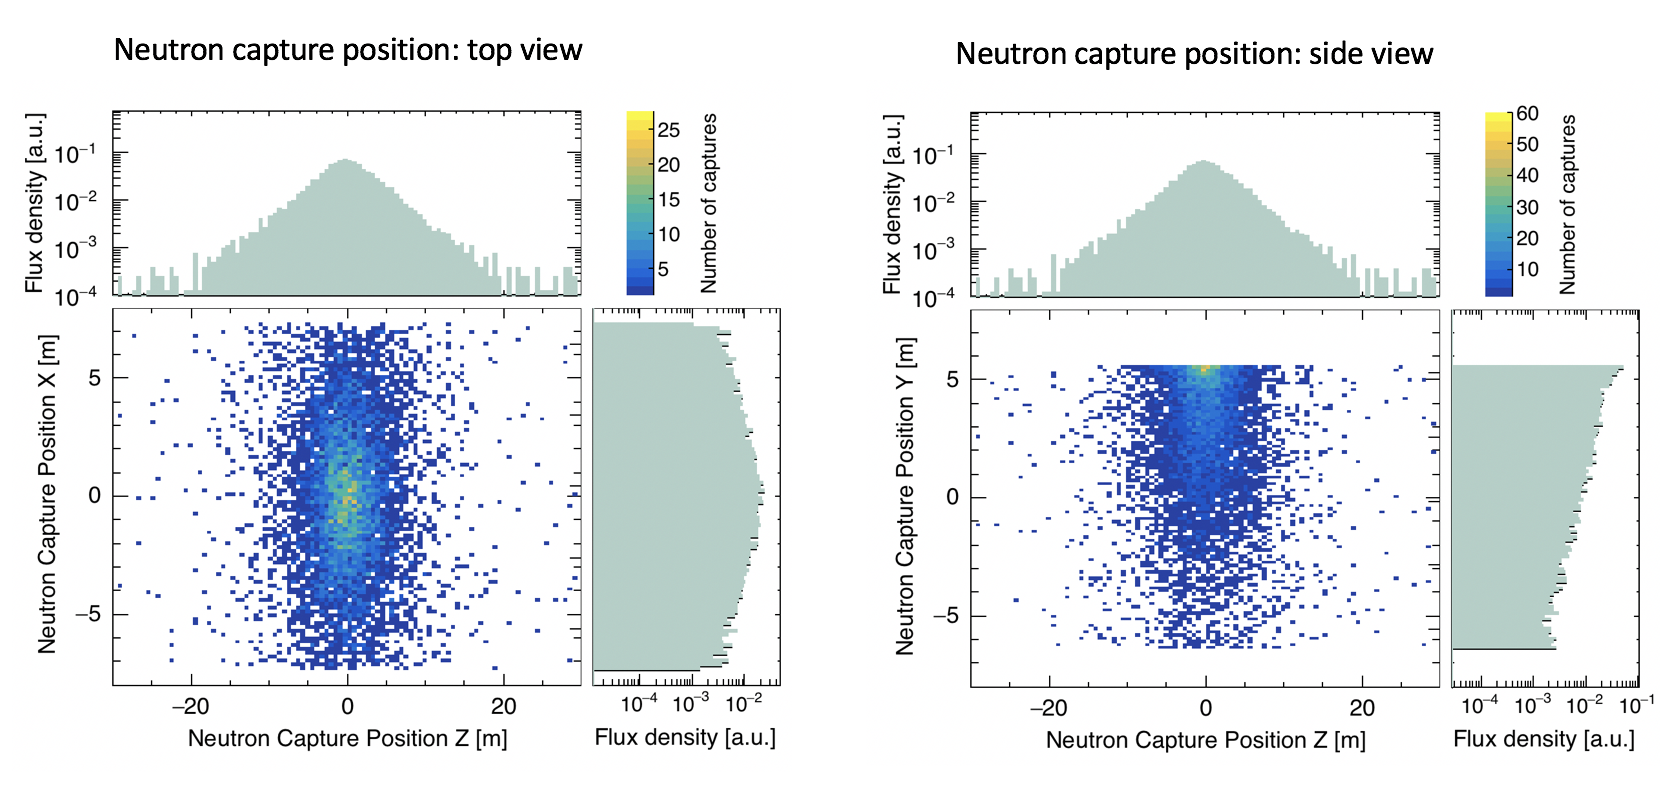
\includegraphics[width=18cm]{PNS_NcapPosition.png}
%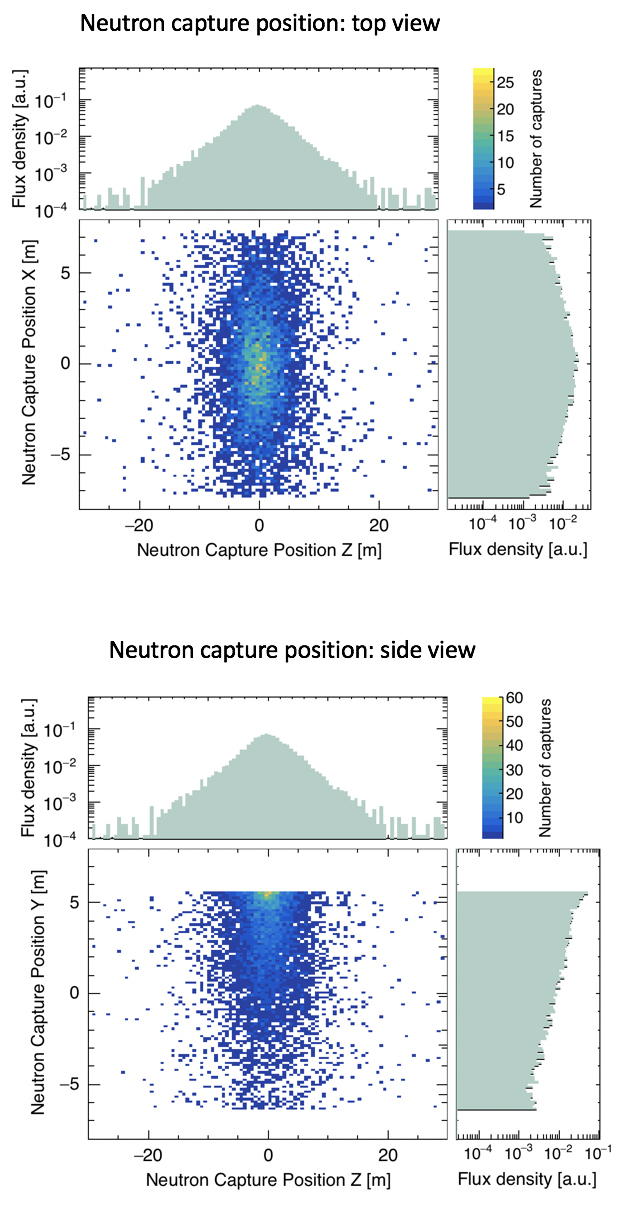
\includegraphics[width=10cm]{PNS_NcapPosition_v2.png}
\end{dunefigure}

%\fixme{SG to Jingbo: Below paragraph is modified. take a look}

The two designs were simulated in GEANT4. Figure~\ref{fig:PNS_NcapPosition} shows the position distribution of the neutron captures. In the simulation, the \dword{pns} is placed on top of the cryostat and is the same size as the \dword{dune} \SI{10}{\kton} \dword{tpc}.  Initial simulation results indicate that one \dword{pns} could cover half the \dword{tpc} volume, so two identical neutron sources, each located at the center of each half of the cryostat
%each central to half the cryostat top,  %\todo{SG: I assume this is with design A, right? if so, mention which design}
would illuminate the whole \dword{tpc} volume of the \dword{dune} \dword{fd} for both designs. This will require two ports, each at 1/4 of the module length (along the beam direction) from each side. This is currently the plan, however exact locations of the ports is yet to be finalized.
%However, this would require opening two additional neutron injection ports which are not included in the current cryostat design \footnote{Ideally, opening two identical neutron injection ports for each \SI{10}{\kton} TPC would make full use of the neutron source. The possibility requires further discussion with the cryostat engineers.}. 
Alternatively, two large format neutron sources (Design A) could be permanently deployed in the human access ports at the corners of the cryostat. One concern in this approach is that the neutrons scattered from the \dword{lar} volume from the human access ports may not reach the center of the \dword{tpc}. This can be mitigated by using a small format neutron source (Design B) deployed on top of the cryostat at the center using the other available instrumentation or calibration feedthroughs. %could be used to complement the coverage of the large format sources. 
In either case, the source will be injected from the top, and neutrons must penetrate the \dword{crp} readout planes, which can reduce the neutron flux going into the \dword{lar}. %\todo{SG to Jingbo: I added the previous sentence, take a look} 
This is currently being investigated.
Figure~\ref{fig:PNS_Energy_Moderator} shows the energy spectrum of the neutrons moderated and injected into the \dword{tpc} based on Design A.
% This figure is based on Design A moderator placed inside the manhole. We can still use this figure, because the energy spectrum shape should be same. Only the flux will be a factor of 6 lower
%The neutron energy is moderated from 2.5 MeV to below 100 keV.  



\begin{dunefigure}[Energy of moderated neutrons produced by the \dlong{pns}]{fig:PNS_Energy_Moderator}
{Energy of moderated neutrons produced by the \dlong{pns}. Simulation is based on Design A. The total number of initial $DD$ generator neutrons is \num{1e6}. }
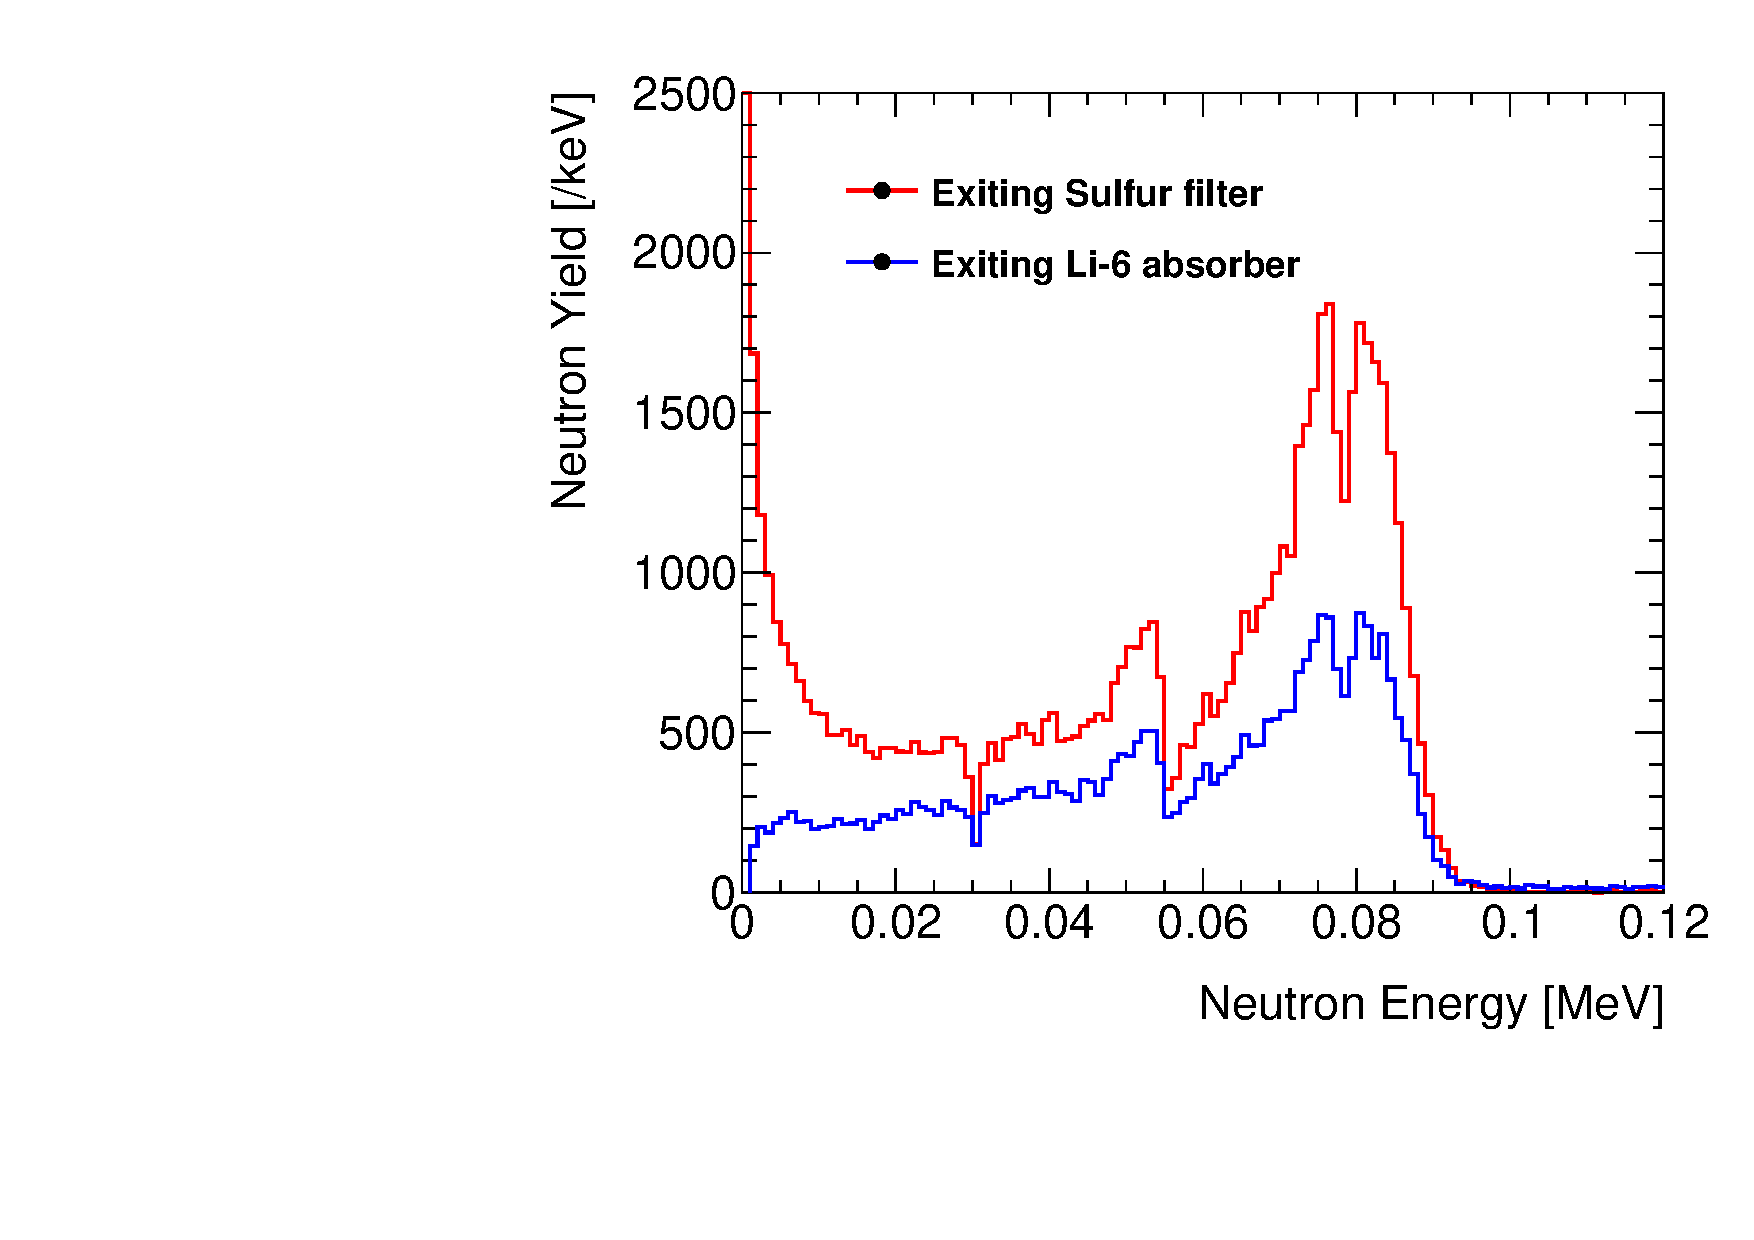
\includegraphics[width=9cm]{PNS_Energy_Moderator.pdf}
\end{dunefigure}

The system should have a long operating lifetime, but because the \dword{pns} system sits on top of the cryostat, with no opening to the \dword{lar}, the system can be replaced if it fails using only crane support.


%%%%%%%%%%%%%%%%%%%%%%%%%%%%
\subsubsection{Measurement Program}
\label{sec:dp-calib-sys-pns-meas}

The \SI{6.1}{\MeV} $\gamma$ cascade will provide a uniform signal for neutron capture, part of the supernova signal. The source may also be used to determine the relative efficiency across the detector for neutron capture, and provide measurements of energy resolution and energy scale spatially and temporally. Simulation studies are currently underway.
%and for the second draft, we plan to include a first round of simulation results.

%\todo{Simulation studies are underway but changing rapidly. for v2 we will include a first round of studies.}

The first goal of the simulation is to provide the expected distribution of signals, with a normalization given by the pulse width of \dword{pns} operation, and neutrons energy and angular correlated distributions, depending on the source filter and shield design.
%, that can also be used to optimize the calibration strategy.
%. It will be used to optimize the calibration strategy too. 
It is envisaged that the calibration can be done in two modes. First, a short \dword{pns} pulse can provide isolated neutron captures closer to the entrance path; and then a longer 
%\dword{pns} 
pulse, for which the same region is saturated, but captures happen in the full volume.
%with isolated neutrons captures obtained in the full volume.

By using an external trigger coupled to the \dword{pns} operation and running the usual trigger algorithms in parallel, the calibration will provide the efficiency of the trigger and \dword{daq} systems as a function of total fluxes. Changing the pulse width can result in 
%resulting on 
higher or lower detector activity. The source will be used for \dword{snb} calibration to test
%, in the sense of testing 
the capabilities of triggering for low energy signals, but also 
%of identifying 
to identify them in different pile-up conditions.
The transmission of the global timing from the external \dword{pns} trigger to the \dword{daq} provides a strong constraint on the initial timing for the \dword{tpc}
%Time Projection Chamber 
as the neutron capture times are of the order of \SI{0.15}{\milli\s}, much lower than typical drift time for the \dword{tpc}. The photon detectors, with resolutions of \SI{100}{\nano\s}, can discriminate between different neutron captures. The calibration will measure the efficiency of the \dword{pds} response for low energy events, depending on the distance due to Rayleigh scattering in \lar. %\fixme{Is this the liquid argon? If so, the dword should be used. Otherwise, in every other place in the manuscript, the scientific abbreviation has been used.}. 
We will then study the usage of the \dword{pds} time information for improving the position reconstruction of \dword{tpc} signals. In the absence of the \dword{pds} system, the global timing from the \dword{pns} translates to an uncertainty of approximately \SI{10}{\cm}.

Individual event positions can be translated into response maps for both the photon detectors and the \dword{lartpc} to standard candles of \SI{6.1}{\MeV} electromagnetic depositions. When the cascades can be more precisely reconstructed, individual $\gamma$s within the cascades can be identified, and this provides a lower energy ``standard candle'' close to the solar electron-neutrino threshold. Comparing the collected charge for equal energy signals at difference distances from the \dword{tpc} gives a measurement of the electron lifetime, a key detector response parameter. High \dword{pns} flux runs can generate momentary local space charge effects, in the
%top parts 
upper regions of the detector must be characterized; low flux runs should be done beforehand to ensure 
%usual 
expected space charge distributions.
The global simulation will be tested in the (smaller scale) \dword{protodune} detectors. The neutron mean free path will be larger than the \dword{protodune} size, and so 
%there will be more 
external events and interactions with materials of the \dword{pds}, \dword{crp}, and \dword{hv} systems will be more prominent. These effects must be simulated.

%Notice 
Note that captures of external background neutrons, entering the active volume is a main background for low energy physics; a comparison of simulations of \dword{pns} events and external neutron backgrounds will be interesting, as will a comparison of simulated supernova and solar neutrino signals. 
%\fixme{Please check the preceding sentence. It was unclear, but I'm not sure I got it right.} 
%\fixme{JM: Re-tweaked, I think it's clearer now. Please remove both if OK.}
For the high energy beam events, the number and energy distributions of neutrons depend on the type of neutrino interaction and are significantly different for neutrinos and anti-neutrinos. Measuring the number and distance of neutron captures around the main hadronic cascades can thus help in identifying which extra proton scattering signals to associate to the hadronic cascades. This can also help make a statistical correction to the energy reconstruction of the neutrino and anti-neutrino events.
%or help in a statistical correction to the energy reconstruction of the neutrino and anti-neutrino events. \fixme{I'm not sure about the clarity of this final sentence either.}
%\fixme{JM: Re-tweaked, I think it's clearer now. Please remove both if OK.}



